\section{Introduction}
\label{section:introduction}




The database, HCI and systems communities have proposed an excess of tools that manage to simplify common tasks that typically take place in an analytical process. Such tools, however, either tend to focus on only individual stages (such as data retrieval or visualization) of a much bigger analytical pipeline or while they do provide a bigger set of possible operations, they only focus on particular use cases (for instance pattern matching, finding correlations and so on). Despite the remarkable contributions, data scientists often have to combine such tools in order to complete an analysis. This lack of flexibility often pushes code-literate data scientists to the tested and proven path of interactive notebooks such as Jupyter.

Interactive notebooks allow the use of popular, high-level and highly expressive imperative languages, such as Python, for retrieving, processing and visualizing data, all in one platform. Due to the high popularity of languages they support, there is also a massive collection of utility libraries that can be used to facilitate any step of a potential data science project. Furthermore, the web environment of notebooks enables collaboration between data scientists, since it allows them to develop and run code, process data and generate visualizations. Lastly, data scientists can compose their findings into an interactive (and re-runnable) report-like page, that contains code, visualizations and textual description of the analysis.

\eat{
Additionally, the notebook-like interface, they offer, enables the creation of interactive documents that contain code, textual description and visualizations, which helps readers follow the analysis and perhaps re-run certain blocks of that notebook.



. Due to the wide popularity of such languages, there is also a huge collection of third-party libraries that can be used by data scientists as building blocks of a much bigger analytical process. Furthermore, the web environment of notebooks enables collaboration between data scientists, since it allows them to directly interact with the user interface in order to develop and run code, process data, generate visualizations, and lastly, compose their findings into an interactive (and re-runnable) report-like page, that contains code, visualizations and textual description of the analysis.
}
However as we show in this work, interactive notebooks are still suboptimal with regard to ease of use and interactivity. Retrieving, processing and visualizing data requires technical knowledge that often exceeds the skill-set of a typical data scientist. Specifically, such steps require transferring files and installing packages to the notebook server, so that they can be used in the analysis. This typically requires knowledge that fits the job description of a system administrator rather than a data analyst. Additionally, even after the environment has been setup, the data analyst has to read long documentation files that explain how to programmatically interact with such tools and often spend significant effort writing plumping code in order combine such tools.


In order to illustrate the challenges, we will use the following example of a potential analysis:

\begin{example}
Consider a data analyst, working for a news portal website, who would like to create a Jupyter notebook that extracts and presents information about the demographics of the website's reader base-during particular hours. More specifically, the analyst would like to construct a chart showing the number of readers that visit the website during the day; then based on this information, she would like to extract the particular age groups that visits the website the most, during specific hours and present this to the portal editor. Figure \ref{fig:vision}a, illustrates the charts that should be created by the data analyst. By doing this, the analyst wishes to convince the portal editor to publish more articles and advertisements that target particular age groups during the hours in which they visit the portal the most, thus maximizing the portal's revenue and user satisfaction.
\end{example}


For this analysis, we assume that the news portal maintains information about its reader-base in a database system. Table \ref{tab:schema} shows a potential database schema, that could have been used for this analysis. The database contains two tables, namely ``Page Views" and ``Visitors", table ``Visitors" stores information about each reader, such as the reader id, name, lastname, and the age, while the table ``Page Views" maintains for each visit a record consisting of a visit id, a reference to the user, and the time in which the user visited the website. This information could have been retrieved, with the users' permission, from various social media services (such as Facebook, Google etc). In order to create this analysis, the data analyst must (a) retrieve  website access information from the database, by joining the two tables on the visitor id (b) generate a plot that shows the number of users that visit the website during the day, (c) issue a query that counts the number of visitors per age group, for each potential set of selected hours, and (d) create a bar chart that shows the number of visitors per age group. 


\subsection{Using Traditional Interactive Notebooks}



In order to perform the afore-mentioned tasks in an interactive notebook that uses python, the data analyst must first install all third-party python packages that will be used for retrieving and visualizing the data. This step will either introduce a dependency between the analyst and some system administrator, or the analyst will need to have the required access rights in order to perform the installation, typically, using a command line. The later can be a security concern or can lead to corrupted systems if not performed correctly. The complexity of this step increases as the number of different database systems, our analyst wants to access, increases. \eat{More specifically, for cases when an analyst needs to access data stored in a MongoDB and a MySQL database, two drivers will need to be installed.}

Once the system is configured, the analyst needs to read lengthy documentation pages in order to properly issue queries to the databases, via imperative code, using the API of the respective library. During this step, the analyst has to also specify the credentials that will be used for accessing the database system. In most such libraries, the credentials have to be inlined into the method that establishes the connection with the database system. While this would not be a security concern in a python application (since the code that includes the credentials would have been compiled into a binary file, thus hiding the credentials), in a Jupyter notebook, the credentials would lie in plain sight for anyone, who has access to the notebook, to see.

After, establishing the connection with the database system, and issuing the queries, the analyst, can consume the results by using the internal, to the library, datamodel. After consuming the results, the analyst will have to again read documentation pages in order to find out how to use the visualization library she selected, then convert the format of the data into the one that is expected by the respective library and lastly construct the first visualization.

The next step, is for the analyst to issue a query that counts the visitors per age group for a set of selected hours and construct a bar chart showing the result. Note, however, that there's no concrete approach for selecting such hours, the analyst will have to go through a process of trial and error, until he finds a set that produces valuable insight. Additionally, even if he does that


Finally, 


plot a line chart of access count Vs timestamp, as well as a bar chart of access count Vs age groups, and (c) be able to select a time range from the line chart using mouse input and automatically filter and display data in the second plot to present age-group-based activity within the selected time frame. 


The data analyst can access historic data about the user base by directly querying the data base system. Table \ref{tab:schema} shows the database schema. The analyst's first task is to retrieve the data via database queries, join the two tables based on the visitor id (``vid'') key and group by (1) ``time'' and (2) ``age'' to prepare the data for the two plots.

Installing packages, transferring data and connecting with database systems requires technical knowledge that often exceeds the skill-set of a typical data scientist. Lastly, while such notebooks support the generation of visualizations with the use of the appropriate library



Throughout this paper, we present {\projname} via an example data analysis: We assume a scenario where a data analyst must (a) retrieve  website access information from a database, (b) plot a line chart of access count Vs timestamp, as well as a bar chart of access count Vs age groups, and (c) be able to select a time range from the line chart using mouse input and automatically filter and display data in the second plot to present age-group-based activity within the selected time frame. 

For our walkthrough example, we assume a Jupyter server where the analysts develop their notebooks and a different database server where data is stored. Table \ref{tab:schema} shows how our databases are organized. The analyst's first task is to retrieve the data via database queries, join the two tables based on the visitor id (``vid'') key and group by (1) ``time'' and (2) ``age'' to prepare the data for the two plots.

During the visualization stage, the analyst implements two ``linked'' plots in such a way that a range selection in the first plot \textit{automatically} (without re-executing code in the notebook) filters the data presented in the second plot. Figure \ref{fig:vision} illustrates the expected chart behavior. A time-frame selection in the first chart (10:00AM - 1:00PM) causes the second chart to only plot those accesses that occurred during the selected interval. 

It is important to note that this interactive chart implementation using imperative languages is not a trivial task and possibly beyond the coding skill set of an average data analyst. Such a task requires advanced coding skills and implementation of event listeners to capture the user's mouse input and asynchronously trigger execution of other functions that will update data and re-draw the second figure. As we show later in Section ??, the {\projname} framework is equipped with modules that can take care of the heavy work, while the analyst only needs to define ``bound'' (linked) variables.

\begin{table}
\begin{center}

\begin{tabular}{|c|c|c|c|}
\hline 
\multicolumn{4}{|c|}{Page Views} \\ 
\hline 
id & vid & url & time \\ 
\hline 
\end{tabular} 

\hfill

\begin{tabular}{|c|c|c|c|c|}
\hline 
\multicolumn{5}{|c|}{Visitors} \\ 
\hline 
vid & name & lastname & username & age \\ 
\hline 
\end{tabular} 

\end{center}
\caption{Schema description of the two tables in our database.}
\label{tab:schema}
\end{table}

The remainder of this paper is organized as follows: Section ?? discusses the architecture of the {\projname} framework. Due to space limitation, we focus on those aspects that can be useful as a notebook extension. Section ?? presents our example data analysis. Finally, Section ?? concludes the paper.

\begin{figure*}
	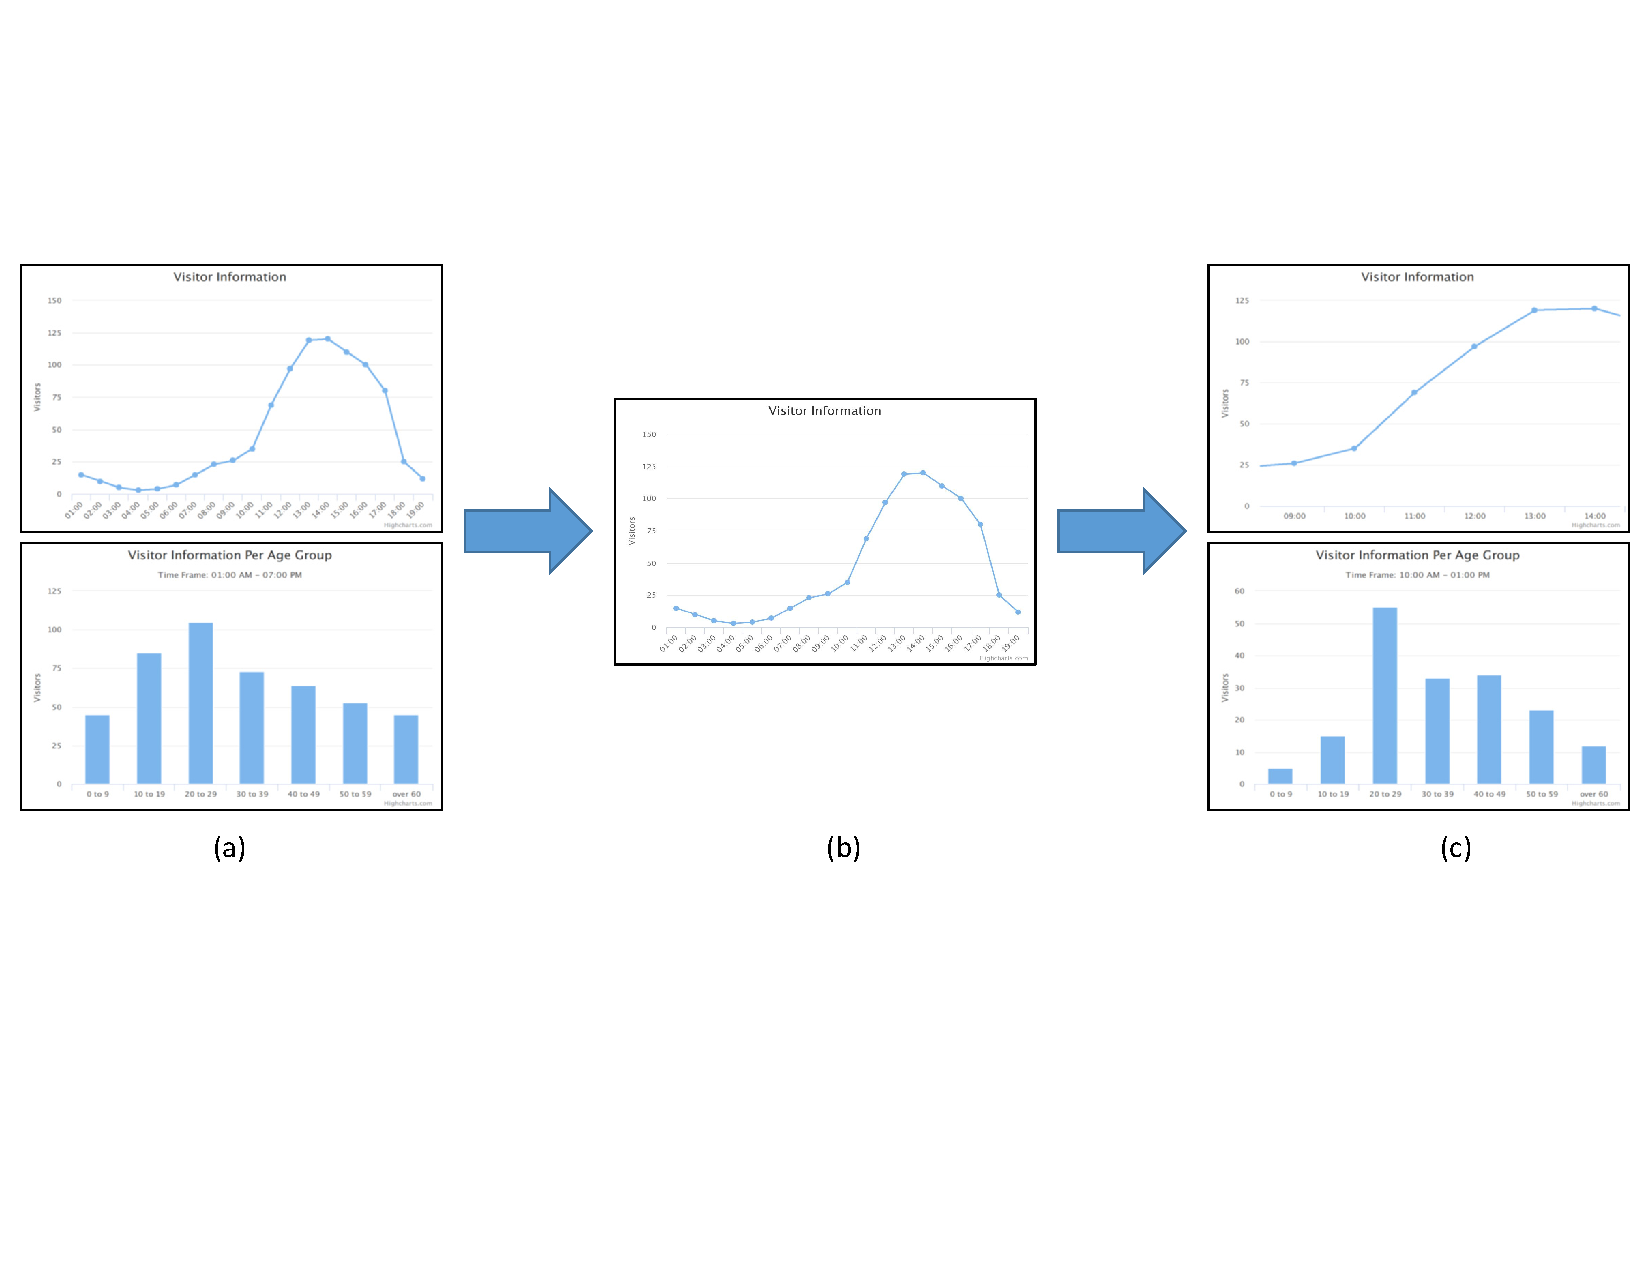
\includegraphics[width=\textwidth]{figures/highchart_final_a.pdf}
	\caption{Demonstration of interactive charts. The analyst's selection automatically updates the second plot (right).}
	\label{fig:vision}
\end{figure*}

\eat{
\begin{figure*}
	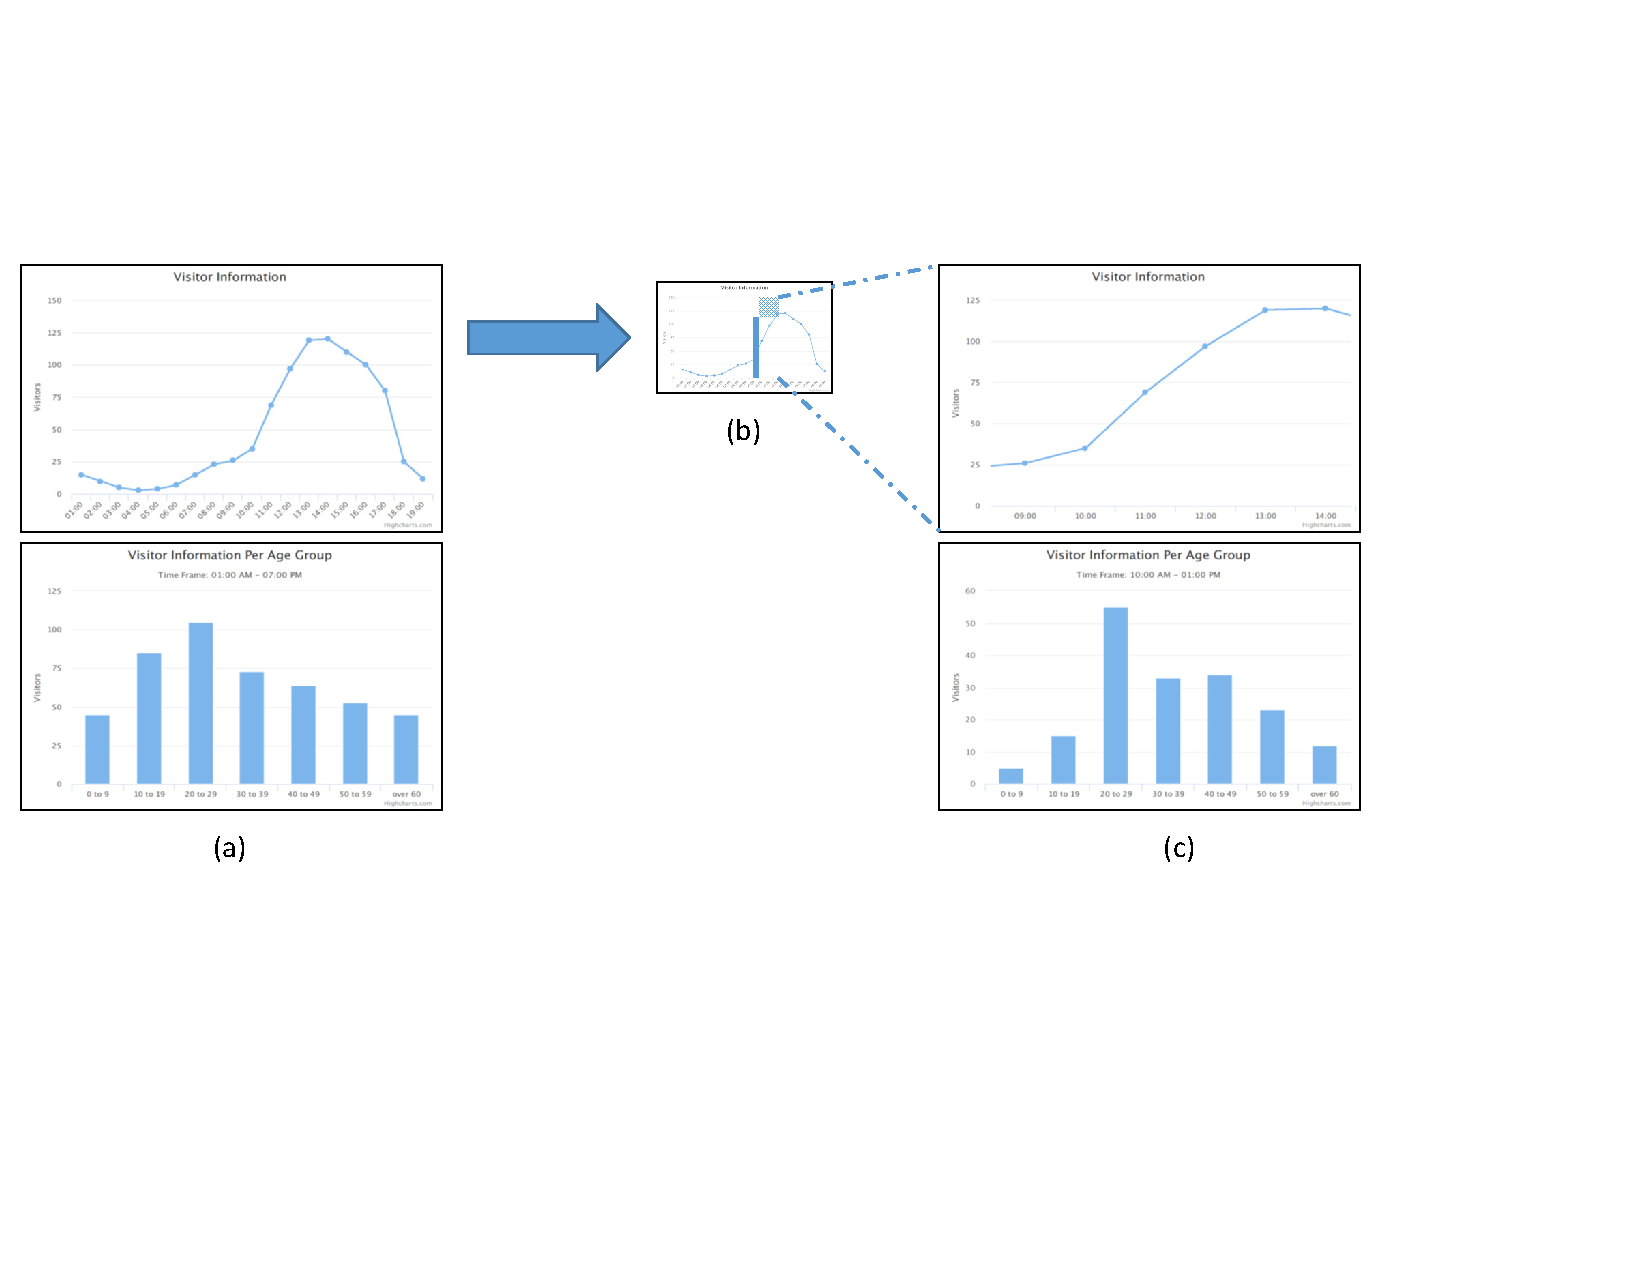
\includegraphics[width=\textwidth]{figures/highchart_final_b.pdf}
	\caption{Demonstration of interactive charts. The analyst's selection automatically updates the second plot (right).}
	\label{fig:vision}
\end{figure*}
}
\remark{Ok I thought about it and I propose the following modifications in the paper structure (Nothing major - just moving text around to make it more readable): We begin with a good discussion about the vidette features that can help notebooks in section 2. We then show the entire walkthrough in one section (Section 3). By now, the reader knows what vidette can do so it will be easier to follow and understand the code we show.}


We address these issues, by extending interactive notebooks with the  {\projname} framework. {\projname} notebooks support a new template language capable of facilitating common data analysis tasks. The main contributions of this extension are:

\begin{itemize}
	\item \textit{Expressive template language:} Prior work, treats a page as a database view. Building on that, our template language goes beyond SQL query and view definition in both style and fundamental expressiveness. It is a mixture of query as well as web templating language that works on ordered (arrays) and semi-ordered (JSON) data. 
	\item \textit{Easy data retrieval:} Our framework supports communication with all major database types, such as Postgress, MongoDB, SQL etc, eliminating the need for individual DB drivers. Furthermore, using {\projname}, user access credentials for the database server(s) are stored in a configuration file, eliminating the embarassingly insecure practice of typing usernames and passwords in notebook cells vidible to everyone.
	\item \textit{Inline JSON operations:} The primary data structure used in {\projname} is JSON arrays. {\projname} combines the intuitive nature of JSON with the ability to write inline JSON operations, resulting in a clean, structured and readable code.
	\item \textit{Variable binding:} Analysts can easily ``bind'' variables using our template language. ``Binding'', results in automatic re-execution of notebook cells that contain those variables upon a change. {\projname} will trigger execution of the appropriate cells without any extra coding effort. As we show later, combined with inline JSON operations, binding becomes an incredibly versatile tool.

%	\item \textit{Declarative semantics:} {\projname} implements formal declarative \textit{Model-View-View-Model} (MVVM) semantics. \remark{Fill in why this is a good thing. I have no idea.}
%	\item \textit{Expressive template language:} Prior database work, treats a page as a database view. Building on that, our template language goes beyond SQL query and view definition in both style and fundamental expressiveness. It is a mixture of query as well as web templating language that works on ordered (arrays) and semi-ordered (JSON) data. 
%	\item We allow in-line declarative code directly in JSON...
\end{itemize}



%In this paper, we demonstrate the use of {\projname} via a walkthrough example. Specifically, we want to use website access data to plot an access count over time histogram. We also want to plot the recorded user demographics (with focus on age groups). We then want to have the ability to interact with the histogram plot and select a time region. This action should automatically update the second plot with the user demographics in the selected time window. 
%
%Without loss of generality, we assume a Jupyter server, where the analysts develop their notebooks and a different database server where data is stored. To retrieve the entirety of the required data, we have to query two different databases and join the returned JSON files. Figure ?? shows how our databases are organized. Our fictional analyst will perform the following high-level tasks:
%
%\begin{itemize}
%	\item Data retrieval from remote databases. 
%	\item Data curation: Join data and prepare for visualization.
%	\item Data visualization.
%\end{itemize}
%
%The remainder of this paper is organized as follows: Sections \ref{section:dataretrieval} -- \ref{section:visualization} present a direct comparison of using {\projname} and an imperative language such as Python in order to complete the tasks of our example. Throughout these sections, we demonstrate some of the main contributions of {\projname}. Section \ref{section:discussion} provides further discussion regarding our proposed extension and presents other useful aspects of it not used in our walkthrough. Finally, Section \ref{section:conclusion} concludes the paper.

